\begin{center}
    \begin{figure}[H]
        \centering

        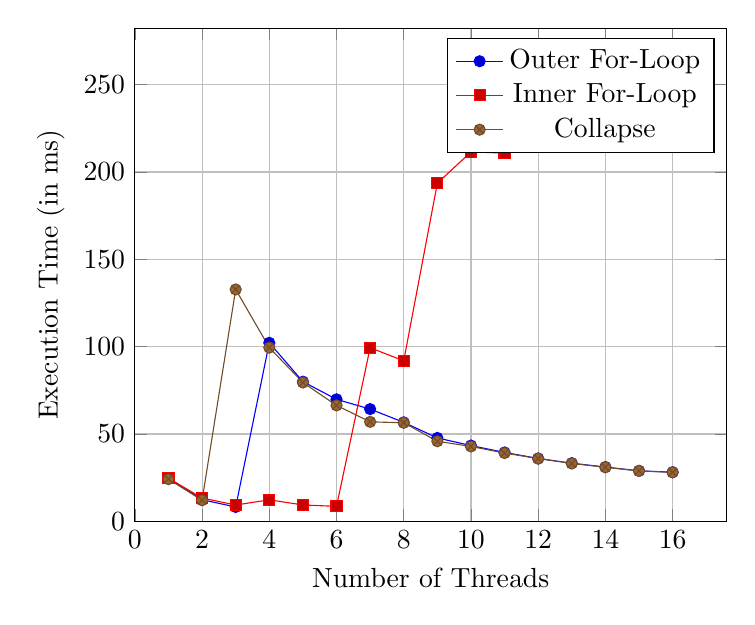
\begin{tikzpicture}
            \begin{axis}[
                title={},
                width=0.75\textwidth,
                xlabel={Number of Threads},
                ylabel={Execution Time (in ms)},
                xmin=0,
                ymin=0,
                grid=major
            ]
                \addplot coordinates {
                    (1,24.661)(2,12.346)(3,8.22125)(4,102.187)(5,79.9541)(6,69.831)(7,64.2403)(8,56.6482)(9,47.7226)(10,43.3734)(11,39.4241)(12,35.9731)(13,33.2708)(14,31.0497)(15,28.8893)(16,28.1236)
                };
                \addlegendentry{Outer For-Loop}

                \addplot coordinates {
                    (1,24.6757)(2,13.3215)(3,9.3242)(4,12.3042)(5,9.3493)(6,8.55875)(7,99.3668)(8,91.8628)(9,193.575)(10,211.472)(11,210.79)(12,219.631)(13,220.46)(14,219.617)(15,245.578)(16,256.618)
                };
                \addlegendentry{Inner For-Loop}       

                \addplot coordinates {
                    (1,24.1217)(2,12.0704)(3,132.73)(4,99.4343)(5,79.4566)(6,66.3546)(7,56.9441)(8,56.4184)(9,45.8333)(10,42.8488)(11,39.0769)(12,35.9021)(13,33.1262)(14,30.931)(15,28.8417)(16,28.0281)
                };
                \addlegendentry{Collapse}
            \end{axis}
        \end{tikzpicture}
        \caption{Grayscale Performance Tests pnglogo-blk.png}
    \end{figure}
\end{center}